\section{java.util.List}

\frame{\frametitle{java.util.List}
\begin{center}
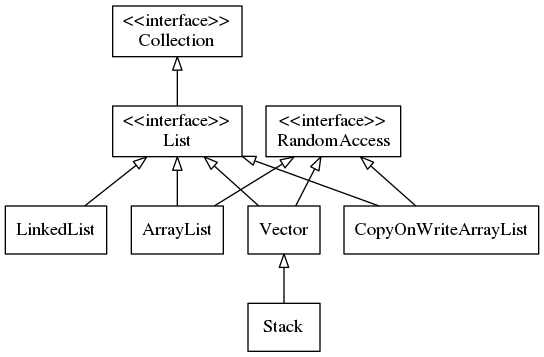
\includegraphics[width=0.9\textwidth]{java.util.List/java_util_List_overview}
\end{center}
}

\frame{
\frametitle{ArrayList}
\begin{center}
  \begin{itemize}[<+->]
    \item Array beinhaltet Elemente
    \item Kapazität kann explizit durch ensureCapacity erhöht werden
    \item fail fast Iterator
    \item quasi ein nicht synchronisierter Vector
    \item null Element erlaubt
    \item remove Operationen verkleinern das Array nicht (trimToSize() verkleinert bis auf die aktuelle Größe)
    \item Re-size Operationen mittels System.arrycopy (nativ, schnell)
    \item TODO 0 bzw. Startgröße, dann jeweils mal 2
    \item remove und add sollten nur am Ende der Liste geschehen
%     \item CPU-cache friendly collection due to being backed by an array 
%     (unfortunately, not too friendly, because contains Objects, which are just 
%     pointers to the actual objects)
    \item nicht thread-safe
  \end{itemize}
\end{center}
}

\frame{
\frametitle{ArrayList - Zugriffszeiten}
\begin{center}
  \begin{tabular}{l|l}
  Operation        & Laufzeit \\\hline
  add              & \O{1} / \O{n} mit re-size \\
  add(int, Object) & je kleiner die Posistion, desto länger \\
  remove(Object)   & \O{n} TODO so viel wegen shifting? was ist shifting? \\
  remove(int)      & \O{n} wegen shifting \\
  get              & \O{1}
  \end{tabular}
\end{center}
}

\frame{
\frametitle{CopyOnWriteArrayList}
\begin{center}
  \begin{itemize}[<+->]
    \item thread-safe Variante von ArrayList
    \item schreibende Operationen (add, set, ...) erstellen eine neue Kopie des Arrays
    \item ''snaphot style iterator''
    \item diese Iteratoren unterstützen keine manipulativen Operationen (UnsupportedOperationException)
    \item null Elemente erlaubt
    \item seit Java 1.5
    \item lesen so teuer wie ArrayList, schreiben teurer wegen der Kopie
  \end{itemize}
\end{center}
}

\frame{
\frametitle{CopyOnWriteArrayList vs Collections.synchronizedList(new ArrayList()}
\begin{center}
  \begin{itemize}[<+->]
    \item synchronizedList synchronisiert immer, auch lesende Zugriffe
    \item Iterator der synchronizedList muss eigenständig synchronisiert werden (fail fast), CopyOneWrite hat fail save
  \end{itemize}
\end{center}
\onslide<+->{$\Rightarrow$ CopyOnWriteArrayList}
}

\frame{
\frametitle{CopyOnWriteArrayList - Wann nehmen?}
\begin{center}
  Wenn man eine ArrayList braucht, \\\pause 
  die thread-safe sein soll, \\\pause 
  mit wenig schreibenden, aber vielen lesenden Zugriffen. \\\pause
  Wenn parallel iteriert werden soll.
\end{center}
}

\frame{
\frametitle{LinkedList}
\begin{center}
  \begin{itemize}[<+->]
    \item double linked
    \item null Elemente erlaubt
    \item Operationen mit Index \O{n}: Traversierung durch gesamte Liste, vorn oder hinten beginnend
    \item nicht thread-safe
    \item fail fast Iterator
    \item Deque Eigenschaften sind herausstechend: addFirst, getFirst, removeFirst, addLast, getLast und removeLast
  \end{itemize}
\end{center}
}

\frame{
\frametitle{LinkedList - Zugriffszeiten}
\begin{center}
  \begin{tabular}{l|l}
  Operation        & Laufzeit \\\hline
  add              & \O{1} \\
  remove(Object)   & \O{1} \\
  remove(int)      & \O{n} \\
  get              & \O{n}
  \end{tabular}
\end{center}
}

\frame{
\frametitle{LinkedList vs ArrayList}
\begin{center}
  \begin{itemize}[<+->]
    \item Laut \href{http://docs.oracle.com/javase/tutorial/collections/implementations/list.html}{Oracle Doku}: ArrayList ist besser
    \item ArrayList mit konstantem Zugriff auf Positionen / Index
    \item ArrayList ist meist schneller: Performance testen, bevor man sich für LinkedList entscheidet
    \item LinkedList erzeugt pro Eintrag ein Node-Object (Overhead)
    \item System.arraycopy muss sehr effizient sein, so dass es ein Vorteil von ArrayList ist
    \item ArrayList hat den Performance-Parameter \textit{initial capacity}
    \item LinkedList ist schneller beim Einfügen vorne und Löschen in der Mitte
    \item Collectors.toList() erstellt eine neue ArrayList
  \end{itemize}
\end{center}
\onslide<+->{$\Rightarrow$ ArrayList}
}

\frame{
\frametitle{LinkedList als Deque}
Folie zuvor: \\
\begin{quotation}
  Deque Eigenschaften sind herausstechend: addFirst, getFirst, removeFirst, addLast, getLast und removeLast \\\pause
\end{quotation}
Aber \href{http://java-performance.info/java-collections-overview/}{Java Performance Tuning Guide} sagt:
\begin{itemize}[<+->]
  \item Wenn man schnellen LinkedList Code schreiben möchte, muss man ListIterators verwenden
  \item Wenn Queue / Deque benötigt wird, lieber ArrayDeque als LinkedList
\end{itemize}
}

\frame{
\frametitle{LinkedList - Wann nehmen?}
\begin{center}
  Wenn sehr oft remove(Object) genutzt wird oder \\\pause
  oft vorne Elemente eingefügt werden. \\\pause
  Kurz: \textbf{Eigentlich gar nicht. Besser ArrayList oder ArrayDeque}
\end{center}
}

\frame{
\frametitle{Stack}
\begin{center}
  \begin{itemize}[<+->]
    \item LIFO: push, pop, peek, search
    \item seit JDK 1.0
  \end{itemize}
\end{center}
}

\frame{
\frametitle{Stack - Wann nehmen?}
\begin{center}
  Ein besseres Interface für LIFO Operationen stellt Deque zur Verfügung: \pause
  \textbf{Gar nicht mehr}
\end{center}
}

\frame{
\frametitle{Vector}
\begin{center}
  \begin{itemize}[<+->]
    \item seit JDK 1.0
    \item wie ein Array (bzw. ArrayList)
    \item thread-safe
    \item alle public Methoden synchronized: einfach, deshalb langsam
    \item fail-fast Iterator
  \end{itemize}
\end{center}
}

\frame{
\frametitle{Vector - Wann nehmen?}
\begin{center}
  \begin{itemize}[<+->]
    \item NIE!
    \item existiert nur noch wegen Abwärtskompatibilität (wurde in Collections ''reingepresst'')
    \item wenn \textbf{kein thread-safe} benötigt wird, dann \textbf{ArrayList}, weil schneller
    \item wenn \textbf{thread-safe} benötigt wird, dann unklar: Vector, Collections.synchronizedList oder CopyOnWriteArrayList
    \item bei Collections.synchronizedList wird zwischen Datenstruktur und Synchronisation getrennt
  \end{itemize}
\end{center}
\begin{center}
  \onslide<+->{$\Rightarrow$ Tendenz ArrayList oder Collections.synchronizedList}
\end{center}
}

\frame{
\frametitle{List - Übersicht}
\begin{center}
  \begin{tabular}{l|c|c|c|c}
                       & thread-safe &  Iterator & Reihenfolge & null value \\\hline
  LinkedList           &             & fail-fast &  insertion  &   erlaubt  \\
  ArrayList            &             & fail-fast &  insertion  &   erlaubt  \\
  Vector               &      ja     & fail-fast &  insertion  &   erlaubt  \\
  Stack                &             & fail-fast &  insertion  &   erlaubt  \\
  CopyOnWriteArrayList &      ja     & fail-safe &  insertion  &   erlaubt  \\
  \end{tabular}
\end{center}
}
